\documentclass{article}
\usepackage[utf8]{inputenc}
\usepackage{hyperref}
\usepackage{graphicx}
\usepackage{float}
\graphicspath{ {./images/} }

\newcommand*\rfrac[2]{{}^{#1}\!/_{#2}}%running fraction with slash - requires math mode.


\title{Catmull-Clark subdivision algorithm}
\author{Michael Spitzer - \href{mailto:vo3xel@gmail.com}{vo3xel@gmail.com}}
\date{February 2019}

\begin{document}

\maketitle

\section{Introduction}
This document describes the application of the Catmull-Clark algorithm on a cube. All steps are available as GeoGebra files.

\section{Catmull-Clark algorithm}
This document is based on the algorithm described in \cite{catmull1978recursively}. The algorithm consists of the following steps:
    \begin{enumerate}
      \item Add face point for each face (average of all original points on face).
      \item Add an edge point for each edge (average of the two neighboring face points and its two original endpoints).
      \item For each face point, add an edge for every edge of the face, connecting the face point to each edge point for the face.
      \item For each original point P, take the average F of all n (recently created) face points for faces touching P, and take the average R of all n edge midpoints for (original) edges touching P, where each edge midpoint is the average of its two endpoint vertices (not to be confused with new "edge points" above). Move each original point to the point:\[P'=\rfrac{F+2R+(n-3)P}{n}\]
      \item Connect each new vertex point to the new edge points of all original edges incident on the original vertex.
    \end{enumerate}
\section{Cube example}
This section describes the application of the algorithm on a simple cube. Figure \ref{fig:cube} shows the cube. The cube has the following vertices:
\[A = \left({\begin{array}{ccc} -1 & -1 & 0 \end{array}}\right) \hspace{10mm} E = \left({\begin{array}{ccc} -1 & -1 & 2 \end{array}}\right) \]
\[B = \left({\begin{array}{ccc} 1  & -1 & 0 \end{array}}\right) \hspace{10mm} F = \left({\begin{array}{ccc}  1 & -1 & 2 \end{array}}\right) \]
\[C = \left({\begin{array}{ccc} 1  &  1 & 0 \end{array}}\right) \hspace{10mm} G = \left({\begin{array}{ccc}  1 &  1 & 2 \end{array}}\right) \]
\[D = \left({\begin{array}{ccc} -1 &  1 & 0 \end{array}}\right) \hspace{10mm} H = \left({\begin{array}{ccc} -1 &  1 & 2 \end{array}}\right) \]
\begin{figure}[H]
\caption{Example cube with length = 2. (GeoGebra link: \href{https://ggbm.at/dfz4phk9}{https://ggbm.at/dfz4phk9})}
\centering
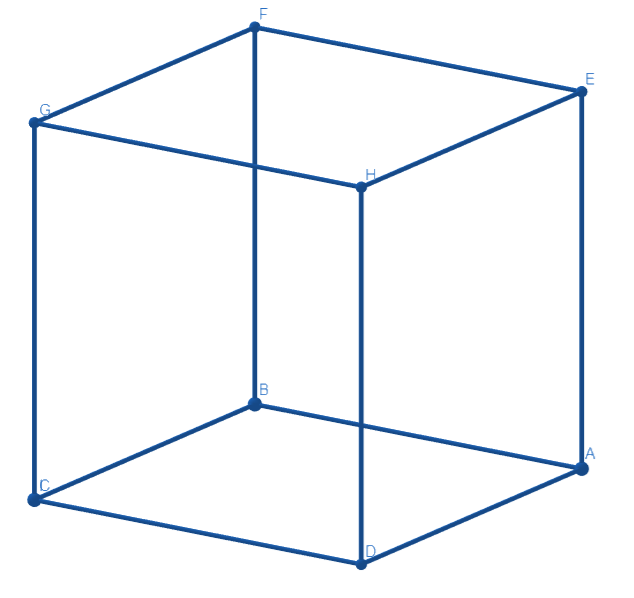
\includegraphics[width=0.8\textwidth]{images/cl-01.png}
\label{fig:cube}
\end{figure}
\subsection{Add face point for each face}
The first step is to compute the face points. The face points are calculated with the following equation: \[f_x=\rfrac{1}{4}\cdot(P_1+P_2+P_3+P_4) \] All four points must be on the same face.
\[f_0=f_{ABCD}=\rfrac{1}{4}\cdot(A+B+C+D)=\rfrac{1}{4}\cdot\left[
\left({\begin{array}{c} -1 \\  -1 \\ 0 \end{array}}\right)+
\left({\begin{array}{c} 1 \\  -1 \\ 0 \end{array}}\right)+
\left({\begin{array}{c} 1 \\  1 \\ 0 \end{array}}\right)+
\left({\begin{array}{c} -1 \\  1 \\ 0 \end{array}}\right)\right]=
\left({\begin{array}{c} 0 \\ 0 \\ 0 \end{array}}\right)
\]
\[f_1=f_{AEFB}=\rfrac{1}{4}\cdot(A+E+F+B)=\rfrac{1}{4}\cdot\left[
\left({\begin{array}{c} -1 \\  -1 \\ 0 \end{array}}\right)+
\left({\begin{array}{c} -1 \\  -1 \\ 2 \end{array}}\right)+
\left({\begin{array}{c} 1 \\  -1 \\ 2 \end{array}}\right)+
\left({\begin{array}{c} 1 \\  -1 \\ 0 \end{array}}\right)\right]=
\left({\begin{array}{c} 0 \\ -1 \\ 1 \end{array}}\right)
\]
\[f_2=f_{BFGC}=\rfrac{1}{4}\cdot(B+F+G+C)=\rfrac{1}{4}\cdot\left[
\left({\begin{array}{c} 1 \\  -1 \\ 0 \end{array}}\right)+
\left({\begin{array}{c} 1 \\  -1 \\ 2 \end{array}}\right)+
\left({\begin{array}{c} 1 \\  1 \\ 2 \end{array}}\right)+
\left({\begin{array}{c} 1 \\  1 \\ 0 \end{array}}\right)\right]=
\left({\begin{array}{c} 1 \\ 0 \\ 1 \end{array}}\right)
\]
\[f_3=f_{CDHG}=\rfrac{1}{4}\cdot(C+D+H+G)=\rfrac{1}{4}\cdot\left[
\left({\begin{array}{c} 1 \\  1 \\ 0 \end{array}}\right)+
\left({\begin{array}{c} -1 \\  1 \\ 0 \end{array}}\right)+
\left({\begin{array}{c} -1 \\  1 \\ 2 \end{array}}\right)+
\left({\begin{array}{c} 1 \\  1 \\ 2 \end{array}}\right)\right]=
\left({\begin{array}{c} 0 \\ 1 \\ 1 \end{array}}\right)
\]
\[f_4=f_{DAEH}=\rfrac{1}{4}\cdot(D+A+E+H)=\rfrac{1}{4}\cdot\left[
\left({\begin{array}{c} -1 \\  1 \\ 0 \end{array}}\right)+
\left({\begin{array}{c} -1 \\ -1 \\ 0 \end{array}}\right)+
\left({\begin{array}{c} -1 \\  -1 \\ 2 \end{array}}\right)+
\left({\begin{array}{c} -1 \\  1 \\ 2 \end{array}}\right)\right]=
\left({\begin{array}{c} -1 \\ 0 \\ 1 \end{array}}\right)
\]
\[f_5=f_{EFGH}=\rfrac{1}{4}\cdot(E+F+G+H)=\rfrac{1}{4}\cdot\left[
\left({\begin{array}{c} -1 \\  -1 \\ 2 \end{array}}\right)+
\left({\begin{array}{c} 1 \\ -1 \\ 2 \end{array}}\right)+
\left({\begin{array}{c} 1 \\  1 \\ 2 \end{array}}\right)+
\left({\begin{array}{c} -1 \\  1 \\ 2 \end{array}}\right)\right]=
\left({\begin{array}{c} 0 \\ 0 \\ 2 \end{array}}\right)
\]
\\
The computed face points are shown in figure \ref{fig:cube2}.
\begin{figure}[H]
\caption{Example cube with computed face points. (GeoGebra link: \href{https://ggbm.at/tmfeuwrn}{https://ggbm.at/tmfeuwrn})}
\centering
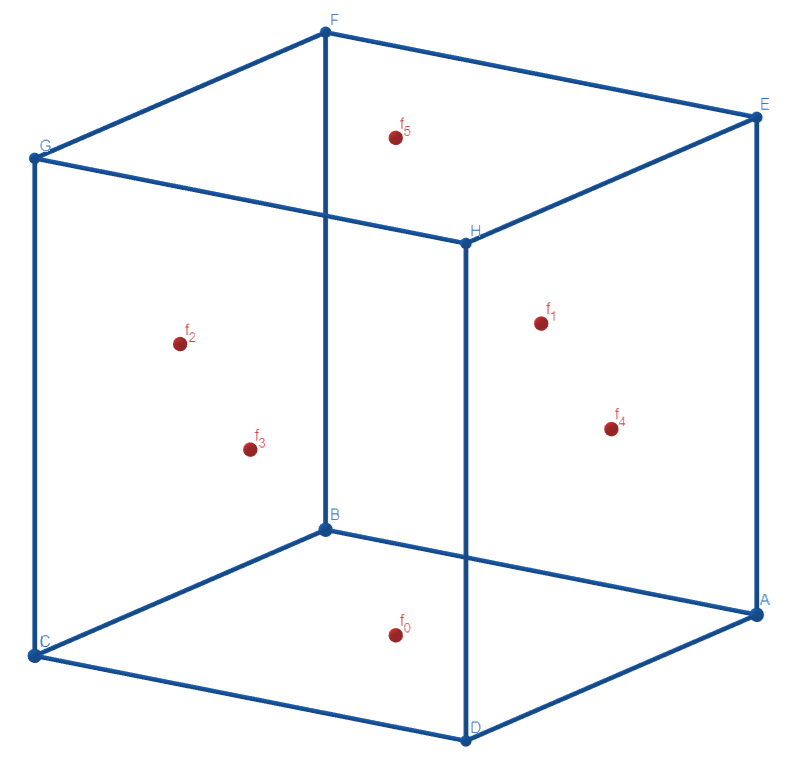
\includegraphics[width=0.8\textwidth]{images/cl-02.png}
\label{fig:cube2}
\end{figure}
\subsection{Add an edge point for each edge}
The edge point is calculated as average of the two neighboring face points and its two original endpoints.
\[e_{P_x,P_y}=\rfrac{1}{4}\cdot(f^{P_x,P_y}_1 + f^{P_x,P_y}_2 + P_x + P_y)\]
The edge point is computed for every line.
\[e_{AB}=\rfrac{1}{4}\cdot(f_0+f_1+A+B)=\rfrac{1}{4}\cdot\left[
\left({\begin{array}{c} 0 \\  0 \\ 0 \end{array}}\right)+
\left({\begin{array}{c} 0 \\ -1 \\ 1 \end{array}}\right)+
\left({\begin{array}{c} -1 \\ -1 \\ 0 \end{array}}\right)+
\left({\begin{array}{c} 1 \\  -1 \\ 0 \end{array}}\right)\right]=
\left({\begin{array}{c} 0 \\ -\rfrac{3}{4} \\ \rfrac{1}{4} \end{array}}\right)
\]
\[e_{BC}=\rfrac{1}{4}\cdot(f_0+f_2+B+C)=\rfrac{1}{4}\cdot\left[
\left({\begin{array}{c} 0 \\  0 \\ 0 \end{array}}\right)+
\left({\begin{array}{c} 1 \\ 0 \\ 1 \end{array}}\right)+
\left({\begin{array}{c} 1 \\ -1 \\ 0 \end{array}}\right)+
\left({\begin{array}{c} 1 \\  1 \\ 0 \end{array}}\right)\right]=
\left({\begin{array}{c} \rfrac{3}{4} \\ 0 \\ \rfrac{1}{4} \end{array}}\right)
\]
\[e_{CD}=\rfrac{1}{4}\cdot(f_0+f_3+C+D)=\rfrac{1}{4}\cdot\left[
\left({\begin{array}{c} 0 \\  0 \\ 0 \end{array}}\right)+
\left({\begin{array}{c} 0 \\ 1 \\ 1 \end{array}}\right)+
\left({\begin{array}{c} 1 \\ 1 \\ 0 \end{array}}\right)+
\left({\begin{array}{c} -1 \\  1 \\ 0 \end{array}}\right)\right]=
\left({\begin{array}{c}  0 \\ \rfrac{3}{4} \\ \rfrac{1}{4} \end{array}}\right)
\]
\[e_{DA}=\rfrac{1}{4}\cdot(f_0+f_4+D+A)=\rfrac{1}{4}\cdot\left[
\left({\begin{array}{c} 0 \\  0 \\ 0 \end{array}}\right)+
\left({\begin{array}{c} -1 \\ 0 \\ 1 \end{array}}\right)+
\left({\begin{array}{c} -1 \\ 1 \\ 0 \end{array}}\right)+
\left({\begin{array}{c} -1 \\  -1 \\ 0 \end{array}}\right)\right]=
\left({\begin{array}{c}  -\rfrac{3}{4} \\ 0 \\ \rfrac{1}{4} \end{array}}\right)
\]
\[e_{AE}=\rfrac{1}{4}\cdot(f_1+f_4+A+E)=\rfrac{1}{4}\cdot\left[
\left({\begin{array}{c} 0 \\  -1 \\ 1 \end{array}}\right)+
\left({\begin{array}{c} -1 \\ 0 \\ 1 \end{array}}\right)+
\left({\begin{array}{c} -1 \\ -1 \\ 0 \end{array}}\right)+
\left({\begin{array}{c} -1 \\  -1 \\ 2 \end{array}}\right)\right]=
\left({\begin{array}{c}  -\rfrac{3}{4} \\ -\rfrac{3}{4} \\ 1 \end{array}}\right)
\]
\[e_{BF}=\rfrac{1}{4}\cdot(f_1+f_2+B+F)=\rfrac{1}{4}\cdot\left[
\left({\begin{array}{c} 0 \\  -1 \\ 1 \end{array}}\right)+
\left({\begin{array}{c} 1 \\ 0 \\ 1 \end{array}}\right)+
\left({\begin{array}{c} 1 \\ -1 \\ 0 \end{array}}\right)+
\left({\begin{array}{c} 1 \\  -1 \\ 2 \end{array}}\right)\right]=
\left({\begin{array}{c}  \rfrac{3}{4} \\ -\rfrac{3}{4} \\ 1 \end{array}}\right)
\]
\[e_{CG}=\rfrac{1}{4}\cdot(f_2+f_3+C+G)=\rfrac{1}{4}\cdot\left[
\left({\begin{array}{c} 1 \\  0 \\ 1 \end{array}}\right)+
\left({\begin{array}{c} 0 \\ 1 \\ 1 \end{array}}\right)+
\left({\begin{array}{c} 1 \\ 1 \\ 0 \end{array}}\right)+
\left({\begin{array}{c} 1 \\  1 \\ 2 \end{array}}\right)\right]=
\left({\begin{array}{c}  \rfrac{3}{4} \\ \rfrac{3}{4} \\ 1 \end{array}}\right)
\]
\[e_{DH}=\rfrac{1}{4}\cdot(f_3+f_4+D+H)=\rfrac{1}{4}\cdot\left[
\left({\begin{array}{c} 0 \\  1 \\ 1 \end{array}}\right)+
\left({\begin{array}{c} -1 \\ 0 \\ 1 \end{array}}\right)+
\left({\begin{array}{c} -1 \\ 1 \\ 0 \end{array}}\right)+
\left({\begin{array}{c} -1 \\  1 \\ 2 \end{array}}\right)\right]=
\left({\begin{array}{c}  -\rfrac{3}{4} \\ \rfrac{3}{4} \\ 1 \end{array}}\right)
\]
\[e_{EF}=\rfrac{1}{4}\cdot(f_1+f_5+E+F)=\rfrac{1}{4}\cdot\left[
\left({\begin{array}{c} 0 \\  -1 \\ 1 \end{array}}\right)+
\left({\begin{array}{c} 0 \\ 0 \\ 2 \end{array}}\right)+
\left({\begin{array}{c} -1 \\ -1 \\ 2 \end{array}}\right)+
\left({\begin{array}{c} 1 \\  -1 \\ 2 \end{array}}\right)\right]=
\left({\begin{array}{c}  0 \\ -\rfrac{3}{4} \\ \rfrac{7}{4} \end{array}}\right)
\]
\[e_{FG}=\rfrac{1}{4}\cdot(f_2+f_5+F+G)=\rfrac{1}{4}\cdot\left[
\left({\begin{array}{c} 1 \\  0 \\ 1 \end{array}}\right)+
\left({\begin{array}{c} 0 \\ 0 \\ 2 \end{array}}\right)+
\left({\begin{array}{c} 1 \\ -1 \\ 2 \end{array}}\right)+
\left({\begin{array}{c} 1 \\  1 \\ 2 \end{array}}\right)\right]=
\left({\begin{array}{c}  \rfrac{3}{4} \\ 0 \\ \rfrac{7}{4} \end{array}}\right)
\]
\[e_{GH}=\rfrac{1}{4}\cdot(f_3+f_5+G+H)=\rfrac{1}{4}\cdot\left[
\left({\begin{array}{c} 0 \\  1 \\ 1 \end{array}}\right)+
\left({\begin{array}{c} 0 \\ 0 \\ 2 \end{array}}\right)+
\left({\begin{array}{c} 1 \\ 1 \\ 2 \end{array}}\right)+
\left({\begin{array}{c} -1 \\  1 \\ 2 \end{array}}\right)\right]=
\left({\begin{array}{c}  0 \\ \rfrac{3}{4} \\ \rfrac{7}{4} \end{array}}\right)
\]
\[e_{HE}=\rfrac{1}{4}\cdot(f_4+f_5+H+E)=\rfrac{1}{4}\cdot\left[
\left({\begin{array}{c} -1 \\  0 \\ 1 \end{array}}\right)+
\left({\begin{array}{c} 0 \\ 0 \\ 2 \end{array}}\right)+
\left({\begin{array}{c} -1 \\ 1 \\ 2 \end{array}}\right)+
\left({\begin{array}{c} -1 \\  -1 \\ 2 \end{array}}\right)\right]=
\left({\begin{array}{c}  -\rfrac{3}{4} \\ 0 \\ \rfrac{7}{4} \end{array}}\right)
\]
\\
The computed edge points are shown in figure \ref{fig:cube3}.
\begin{figure}[H]
\caption{Example cube with computed edge points. (GeoGebra link: \href{https://ggbm.at/kmwfec2m}{https://ggbm.at/kmwfec2m})}
\centering
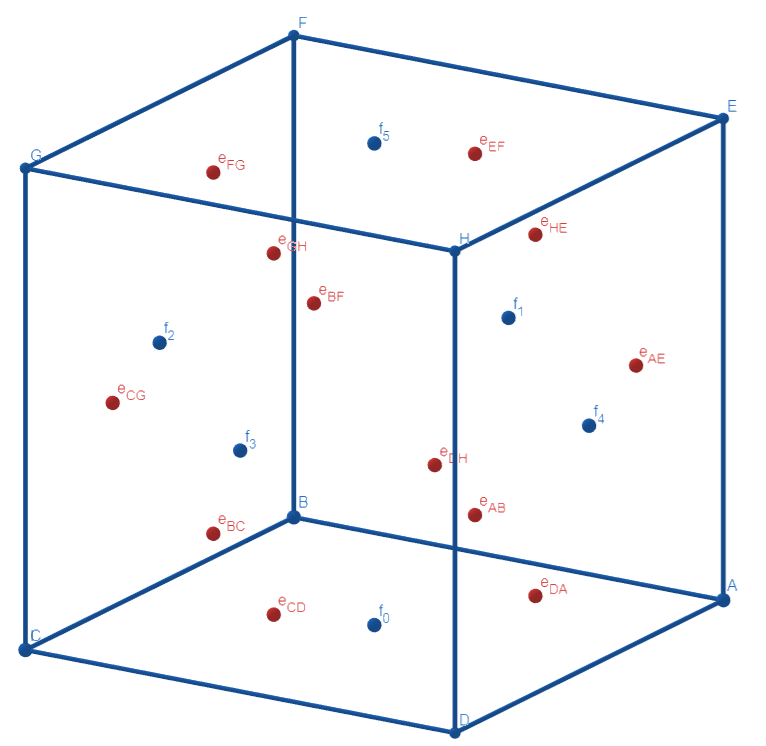
\includegraphics[width=0.8\textwidth]{images/cl-03.png}
\label{fig:cube3}
\end{figure}
\subsection{Connect face points and face vertices with edges}
Figure \ref{fig:cube4} shows the face points connected with face vertices.
\begin{figure}[H]
\caption{Example cube with computed edge points. (GeoGebra link: \href{https://ggbm.at/ungtevwr}{https://ggbm.at/ungtevwr})}
\centering
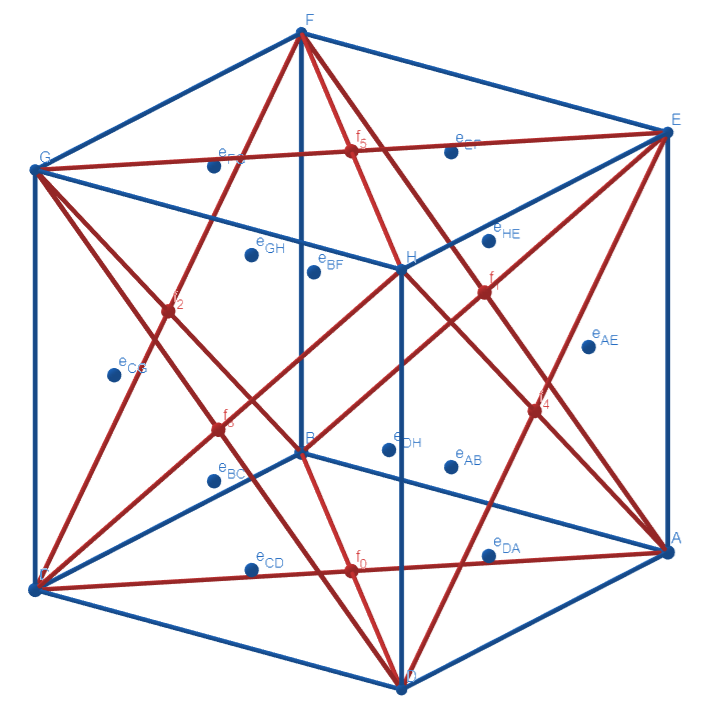
\includegraphics[width=0.8\textwidth]{images/cl-04.png}
\label{fig:cube4}
\end{figure}
\subsection{Move each original point}
Move each original point to the point:\[P'=\rfrac{F+2R+(n-3)P}{n}\]
Since the shape is a cube (n=3) the equation can be simplified to:\[P'=\rfrac{F+2R}{3}\]
(F ... average of all face points of faces touching P, R ... average of all edge mid points of edges touching P, n ... number of faces touching the point, P ... original point)

\subsubsection{Compute edge mid points}
\[em_{P_x,P_y}=\rfrac{1}{2}\cdot(P_x+P_y)\]
\[em_{AB}=\rfrac{1}{2}\cdot(A+B)=\rfrac{1}{2}\cdot\left[
\left({\begin{array}{c} -1 \\  -1 \\ 0 \end{array}}\right)+
\left({\begin{array}{c} 1 \\  -1 \\ 0 \end{array}}\right)\right]=
\left({\begin{array}{c}  0 \\ -1 \\ 0 \end{array}}\right)
\]
\[em_{BC}=\rfrac{1}{2}\cdot(B+C)=\rfrac{1}{2}\cdot\left[
\left({\begin{array}{c} 1 \\  -1 \\ 0 \end{array}}\right)+
\left({\begin{array}{c} 1 \\  1 \\ 0 \end{array}}\right)\right]=
\left({\begin{array}{c}  1 \\ 0 \\ 0 \end{array}}\right)
\]
\[em_{CD}=\rfrac{1}{2}\cdot(C+D)=\rfrac{1}{2}\cdot\left[
\left({\begin{array}{c} 1 \\  1 \\ 0 \end{array}}\right)+
\left({\begin{array}{c} -1 \\  1 \\ 0 \end{array}}\right)\right]=
\left({\begin{array}{c}  0 \\ 1 \\ 0 \end{array}}\right)
\]
\[em_{DA}=\rfrac{1}{2}\cdot(D+A)=\rfrac{1}{2}\cdot\left[
\left({\begin{array}{c} -1 \\  1 \\ 0 \end{array}}\right)+
\left({\begin{array}{c} -1 \\  -1 \\ 0 \end{array}}\right)\right]=
\left({\begin{array}{c}  -1 \\ 0 \\ 0 \end{array}}\right)
\]
\[em_{AE}=\rfrac{1}{2}\cdot(A+E)=\rfrac{1}{2}\cdot\left[
\left({\begin{array}{c} -1 \\  -1 \\ 0 \end{array}}\right)+
\left({\begin{array}{c} -1 \\  -1 \\ 2 \end{array}}\right)\right]=
\left({\begin{array}{c} -1 \\ -1 \\ 1 \end{array}}\right)
\]
\[em_{BF}=\rfrac{1}{2}\cdot(B+F)=\rfrac{1}{2}\cdot\left[
\left({\begin{array}{c} 1 \\  -1 \\ 0 \end{array}}\right)+
\left({\begin{array}{c} 1 \\  -1 \\ 2 \end{array}}\right)\right]=
\left({\begin{array}{c} 1 \\ -1 \\ 1 \end{array}}\right)
\]
\[em_{CG}=\rfrac{1}{2}\cdot(C+G)=\rfrac{1}{2}\cdot\left[
\left({\begin{array}{c} 1 \\  1 \\ 0 \end{array}}\right)+
\left({\begin{array}{c} 1 \\  1 \\ 2 \end{array}}\right)\right]=
\left({\begin{array}{c} 1 \\ 1 \\ 1 \end{array}}\right)
\]
\[em_{DH}=\rfrac{1}{2}\cdot(D+H)=\rfrac{1}{2}\cdot\left[
\left({\begin{array}{c} -1 \\  1 \\ 0 \end{array}}\right)+
\left({\begin{array}{c} -1 \\  1 \\ 2 \end{array}}\right)\right]=
\left({\begin{array}{c} -1 \\ 1 \\ 1 \end{array}}\right)
\]
\[em_{EF}=\rfrac{1}{2}\cdot(E+F)=\rfrac{1}{2}\cdot\left[
\left({\begin{array}{c} -1 \\  -1 \\ 2 \end{array}}\right)+
\left({\begin{array}{c} 1 \\  -1 \\ 2 \end{array}}\right)\right]=
\left({\begin{array}{c} 0 \\ -1 \\ 2 \end{array}}\right)
\]
\[em_{FG}=\rfrac{1}{2}\cdot(F+G)=\rfrac{1}{2}\cdot\left[
\left({\begin{array}{c} 1 \\  -1 \\ 2 \end{array}}\right)+
\left({\begin{array}{c} 1 \\  1 \\ 2 \end{array}}\right)\right]=
\left({\begin{array}{c} 1 \\ 0 \\ 2 \end{array}}\right)
\]
\[em_{GH}=\rfrac{1}{2}\cdot(G+H)=\rfrac{1}{2}\cdot\left[
\left({\begin{array}{c} 1 \\  1 \\ 2 \end{array}}\right)+
\left({\begin{array}{c} -1 \\  1 \\ 2 \end{array}}\right)\right]=
\left({\begin{array}{c} 0 \\ 1 \\ 2 \end{array}}\right)
\]
\[em_{HE}=\rfrac{1}{2}\cdot(H+E)=\rfrac{1}{2}\cdot\left[
\left({\begin{array}{c} -1 \\  1 \\ 2 \end{array}}\right)+
\left({\begin{array}{c} -1 \\  -1 \\ 2 \end{array}}\right)\right]=
\left({\begin{array}{c} -1 \\ 0 \\ 2 \end{array}}\right)
\]
\\
Figure \ref{fig:cube5} shows the computed edge points.
\begin{figure}[H]
\caption{Example cube with computed edge mid points. (GeoGebra link: \href{https://ggbm.at/ng8zqgpr}{https://ggbm.at/ng8zqgpr})}
\centering
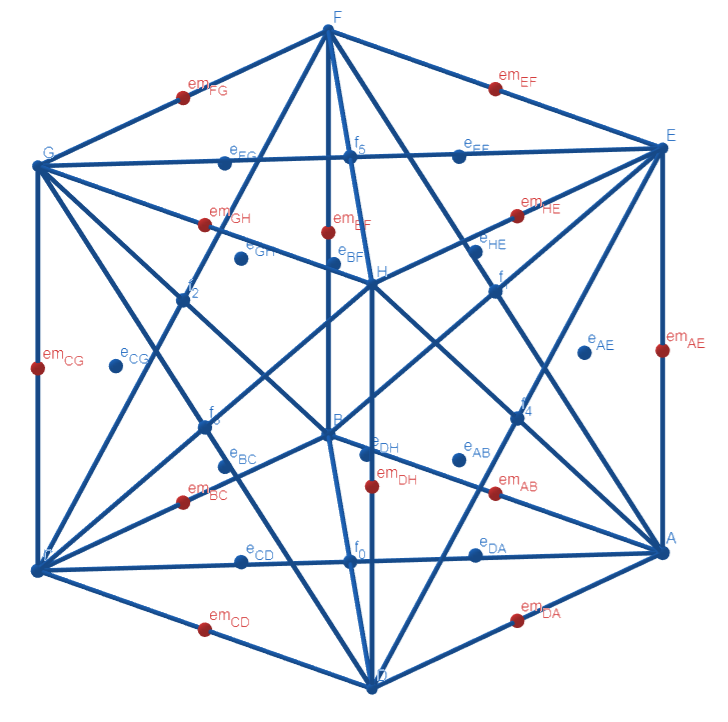
\includegraphics[width=0.8\textwidth]{images/cl-05.png}
\label{fig:cube5}
\end{figure}

\subsubsection{Move original vertices}
\[P'=\rfrac{F+2R}{3}\]
\[A'=\rfrac{\rfrac{1}{3}\cdot\left[f_0+f_1+f_4\right]+
\rfrac{2}{3}\cdot\left[em_{AB}+em_{DA}+em_{AE}\right]
}{3}\]
\[A'=\rfrac{\rfrac{1}{3}\cdot\left[
\left({\begin{array}{c} 0 \\  0 \\ 0 \end{array}}\right)+
\left({\begin{array}{c} 0 \\  -1 \\ 1 \end{array}}\right)+
\left({\begin{array}{c} -1 \\  0 \\ 1 \end{array}}\right)\right]+
\rfrac{2}{3}\cdot\left[
\left({\begin{array}{c} 0 \\  -1 \\ 0 \end{array}}\right)+
\left({\begin{array}{c} -1 \\  0 \\ 0 \end{array}}\right)+
\left({\begin{array}{c} -1 \\  -1 \\ 1 \end{array}}\right)\right]
}{3}=\left({\begin{array}{c} -\rfrac{5}{9} \\  -\rfrac{5}{9} \\ \rfrac{4}{9} \end{array}}\right)\]
\[B'=\rfrac{\rfrac{1}{3}\cdot\left[f_0+f_1+f_2\right]+
\rfrac{2}{3}\cdot\left[em_{AB}+em_{BC}+em_{BF}\right]
}{3}\]
\[B'=\rfrac{\rfrac{1}{3}\cdot\left[
\left({\begin{array}{c} 0 \\  0 \\ 0 \end{array}}\right)+
\left({\begin{array}{c} 0 \\  -1 \\ 1 \end{array}}\right)+
\left({\begin{array}{c} 1 \\  0 \\ 1 \end{array}}\right)\right]+
\rfrac{2}{3}\cdot\left[
\left({\begin{array}{c} 0 \\  -1 \\ 0 \end{array}}\right)+
\left({\begin{array}{c} 1 \\  0 \\ 0 \end{array}}\right)+
\left({\begin{array}{c} 1 \\  -1 \\ 1 \end{array}}\right)\right]
}{3}=\left({\begin{array}{c} \rfrac{5}{9} \\  -\rfrac{5}{9} \\ \rfrac{4}{9} \end{array}}\right)\]
\[C'=\rfrac{\rfrac{1}{3}\cdot\left[f_0+f_2+f_3\right]+
\rfrac{2}{3}\cdot\left[em_{BC}+em_{CD}+em_{CG}\right]
}{3}\]
\[C'=\rfrac{\rfrac{1}{3}\cdot\left[
\left({\begin{array}{c} 0 \\  0 \\ 0 \end{array}}\right)+
\left({\begin{array}{c} 1 \\  0 \\ 1 \end{array}}\right)+
\left({\begin{array}{c} 0 \\  1 \\ 1 \end{array}}\right)\right]+
\rfrac{2}{3}\cdot\left[
\left({\begin{array}{c} 1 \\  0 \\ 0 \end{array}}\right)+
\left({\begin{array}{c} 0 \\  1 \\ 0 \end{array}}\right)+
\left({\begin{array}{c} 1 \\  1 \\ 1 \end{array}}\right)\right]
}{3}=\left({\begin{array}{c} \rfrac{5}{9} \\  \rfrac{5}{9} \\ \rfrac{4}{9} \end{array}}\right)\]
\[D'=\rfrac{\rfrac{1}{3}\cdot\left[f_0+f_3+f_4\right]+
\rfrac{2}{3}\cdot\left[em_{CD}+em_{DA}+em_{DH}\right]
}{3}\]
\[D'=\rfrac{\rfrac{1}{3}\cdot\left[
\left({\begin{array}{c} 0 \\  0 \\ 0 \end{array}}\right)+
\left({\begin{array}{c} 0 \\  1 \\ 1 \end{array}}\right)+
\left({\begin{array}{c} -1 \\  0 \\ 1 \end{array}}\right)\right]+
\rfrac{2}{3}\cdot\left[
\left({\begin{array}{c} 0 \\  1 \\ 0 \end{array}}\right)+
\left({\begin{array}{c} -1 \\  0 \\ 0 \end{array}}\right)+
\left({\begin{array}{c} -1 \\  1 \\ 1 \end{array}}\right)\right]
}{3}=\left({\begin{array}{c} -\rfrac{5}{9} \\  \rfrac{5}{9} \\ \rfrac{4}{9} \end{array}}\right)\]
\[E'=\rfrac{\rfrac{1}{3}\cdot\left[f_1+f_4+f_5\right]+
\rfrac{2}{3}\cdot\left[em_{AE}+em_{EF}+em_{HE}\right]
}{3}\]
\[E'=\rfrac{\rfrac{1}{3}\cdot\left[
\left({\begin{array}{c} 0 \\  -1 \\ 1 \end{array}}\right)+
\left({\begin{array}{c} -1 \\  0 \\ 1 \end{array}}\right)+
\left({\begin{array}{c} 0 \\  0 \\ 2 \end{array}}\right)\right]+
\rfrac{2}{3}\cdot\left[
\left({\begin{array}{c} -1 \\  -1 \\ 1 \end{array}}\right)+
\left({\begin{array}{c} 0 \\  -1 \\ 2 \end{array}}\right)+
\left({\begin{array}{c} -1 \\  0 \\ 2 \end{array}}\right)\right]
}{3}=\left({\begin{array}{c} -\rfrac{5}{9} \\  -\rfrac{5}{9} \\ \rfrac{14}{9} \end{array}}\right)\]
\[F'=\rfrac{\rfrac{1}{3}\cdot\left[f_1+f_2+f_5\right]+
\rfrac{2}{3}\cdot\left[em_{BF}+em_{FG}+em_{EF}\right]
}{3}\]
\[F'=\rfrac{\rfrac{1}{3}\cdot\left[
\left({\begin{array}{c} 0 \\  -1 \\ 1 \end{array}}\right)+
\left({\begin{array}{c} 1 \\  0 \\ 1 \end{array}}\right)+
\left({\begin{array}{c} 0 \\  0 \\ 2 \end{array}}\right)\right]+
\rfrac{2}{3}\cdot\left[
\left({\begin{array}{c} 1 \\  -1 \\ 1 \end{array}}\right)+
\left({\begin{array}{c} 1 \\  0 \\ 2 \end{array}}\right)+
\left({\begin{array}{c} 0 \\  -1 \\ 2 \end{array}}\right)\right]
}{3}=\left({\begin{array}{c} \rfrac{5}{9} \\  -\rfrac{5}{9} \\ \rfrac{14}{9} \end{array}}\right)\]
\[G'=\rfrac{\rfrac{1}{3}\cdot\left[f_2+f_3+f_5\right]+
\rfrac{2}{3}\cdot\left[em_{CG}+em_{FG}+em_{GH}\right]
}{3}\]
\[G'=\rfrac{\rfrac{1}{3}\cdot\left[
\left({\begin{array}{c} 1 \\  0 \\ 1 \end{array}}\right)+
\left({\begin{array}{c} 0 \\  1 \\ 1 \end{array}}\right)+
\left({\begin{array}{c} 0 \\  0 \\ 2 \end{array}}\right)\right]+
\rfrac{2}{3}\cdot\left[
\left({\begin{array}{c} 1 \\  1 \\ 1 \end{array}}\right)+
\left({\begin{array}{c} 1 \\  0 \\ 2 \end{array}}\right)+
\left({\begin{array}{c} 0 \\  1 \\ 2 \end{array}}\right)\right]
}{3}=\left({\begin{array}{c} \rfrac{5}{9} \\  \rfrac{5}{9} \\ \rfrac{14}{9} \end{array}}\right)\]
\[H'=\rfrac{\rfrac{1}{3}\cdot\left[f_3+f_4+f_5\right]+
\rfrac{2}{3}\cdot\left[em_{DH}+em_{GH}+em_{HE}\right]
}{3}\]
\[H'=\rfrac{\rfrac{1}{3}\cdot\left[
\left({\begin{array}{c} 0 \\  1 \\ 1 \end{array}}\right)+
\left({\begin{array}{c} -1 \\  0 \\ 1 \end{array}}\right)+
\left({\begin{array}{c} 0 \\  0 \\ 2 \end{array}}\right)\right]+
\rfrac{2}{3}\cdot\left[
\left({\begin{array}{c} -1 \\  1 \\ 1 \end{array}}\right)+
\left({\begin{array}{c} -1 \\  0 \\ 2 \end{array}}\right)+
\left({\begin{array}{c} 0 \\  1 \\ 2 \end{array}}\right)\right]
}{3}=\left({\begin{array}{c} -\rfrac{5}{9} \\  \rfrac{5}{9} \\ \rfrac{14}{9} \end{array}}\right)\]
Figure \ref{fig:cube6} shows the moved vertices.
\begin{figure}[H]
\caption{Example cube with moved vertices. (GeoGebra link: \href{https://ggbm.at/s9s9jbta}{https://ggbm.at/s9s9jbta})}
\centering
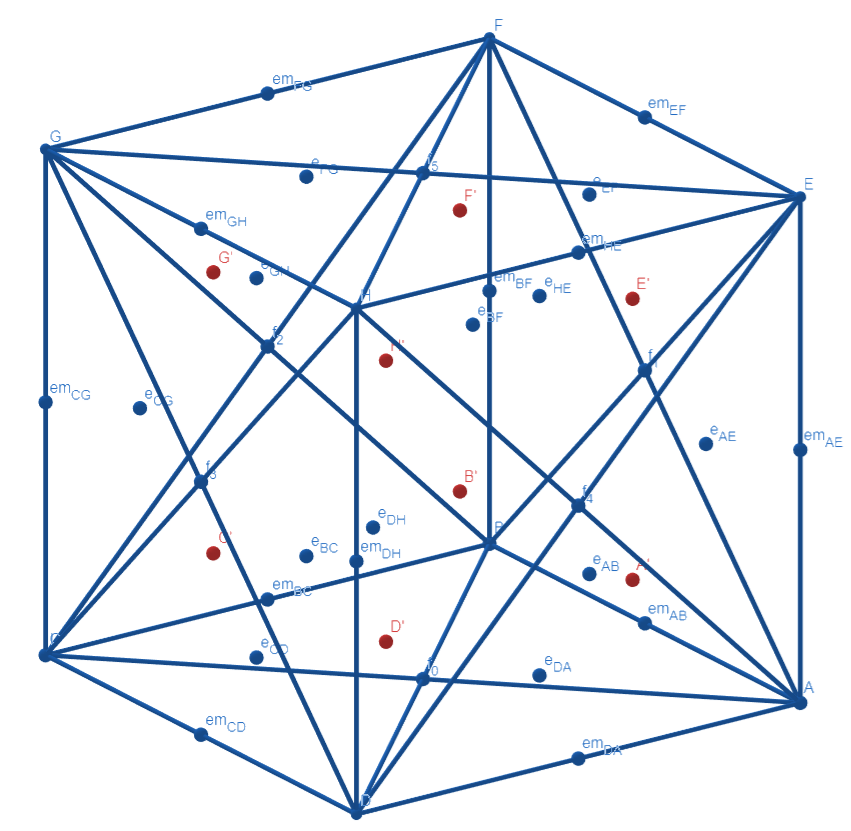
\includegraphics[width=0.8\textwidth]{images/cl-06.png}
\label{fig:cube6}
\end{figure}
\subsection{Connect each new vertex point}
Connect each new vertex point to the new edge points of all original edges incident on the original vertex.
\subsubsection{A \rightarrow A'}
\begin{figure}[H]
\caption{A' (GeoGebra link: \href{https://ggbm.at/u7rp4pe8}{https://ggbm.at/u7rp4pe8})}
\centering
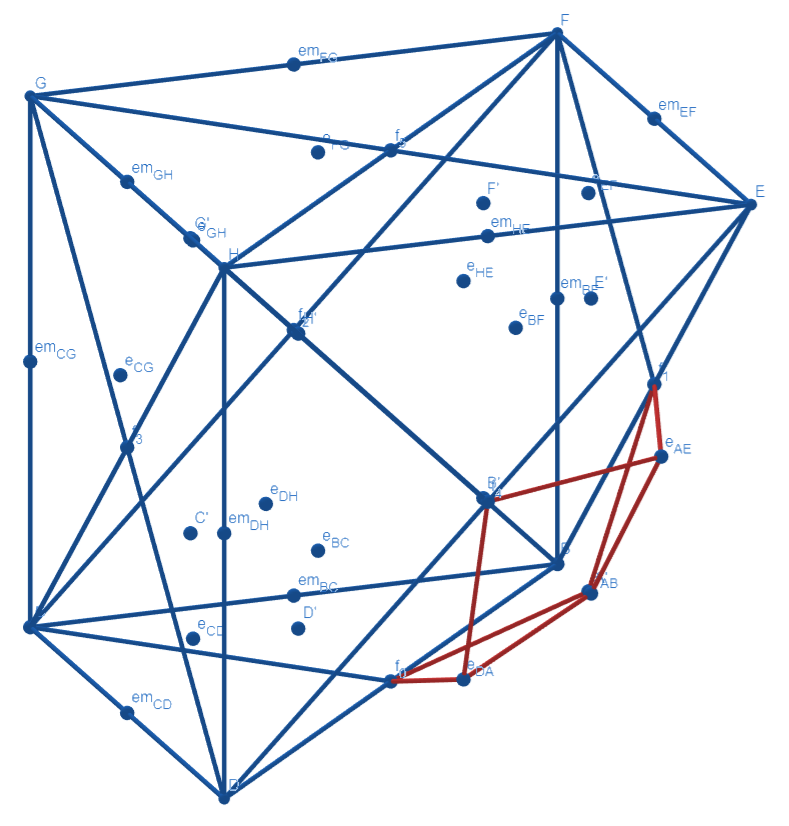
\includegraphics[width=0.8\textwidth]{images/cl-07-1.png}
\label{fig:cube7-1}
\end{figure}
\subsubsection{B \rightarrow B'}
\begin{figure}[H]
\caption{B' (GeoGebra link: \href{https://ggbm.at/se5hwy89}{https://ggbm.at/se5hwy89})}
\centering
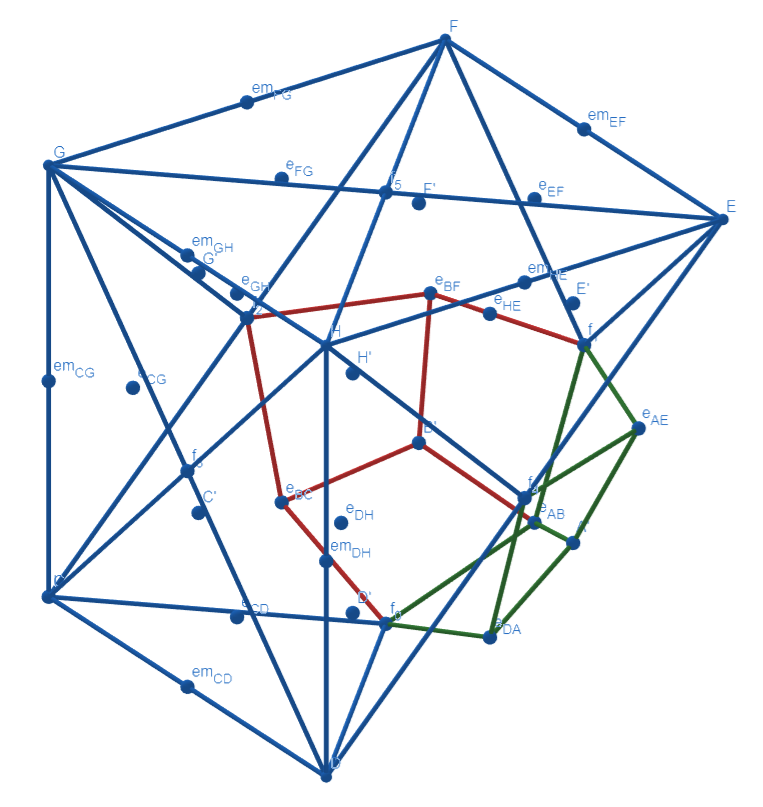
\includegraphics[width=0.8\textwidth]{images/cl-07-2.png}
\label{fig:cube7-2}
\end{figure}
\subsubsection{C \rightarrow C'}
\begin{figure}[H]
\caption{C' (GeoGebra link: \href{https://ggbm.at/vwx3rxrm}{https://ggbm.at/vwx3rxrm})}
\centering
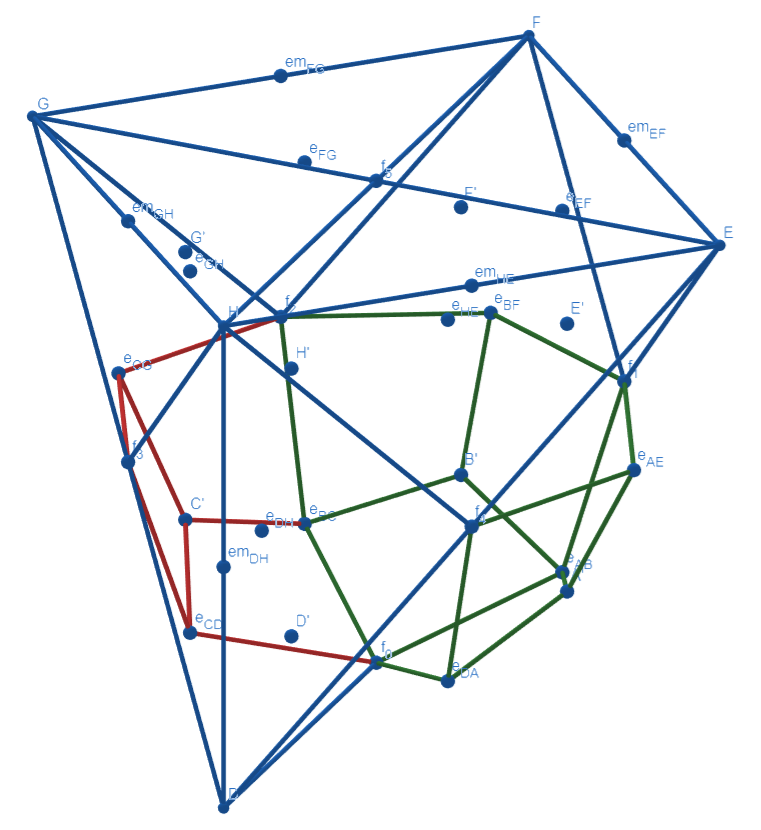
\includegraphics[width=0.8\textwidth]{images/cl-07-3.png}
\label{fig:cube7-3}
\end{figure}
\subsubsection{D \rightarrow D'}
\begin{figure}[H]
\caption{D' (GeoGebra link: \href{https://ggbm.at/u4hnhdtc}{https://ggbm.at/u4hnhdtc})}
\centering
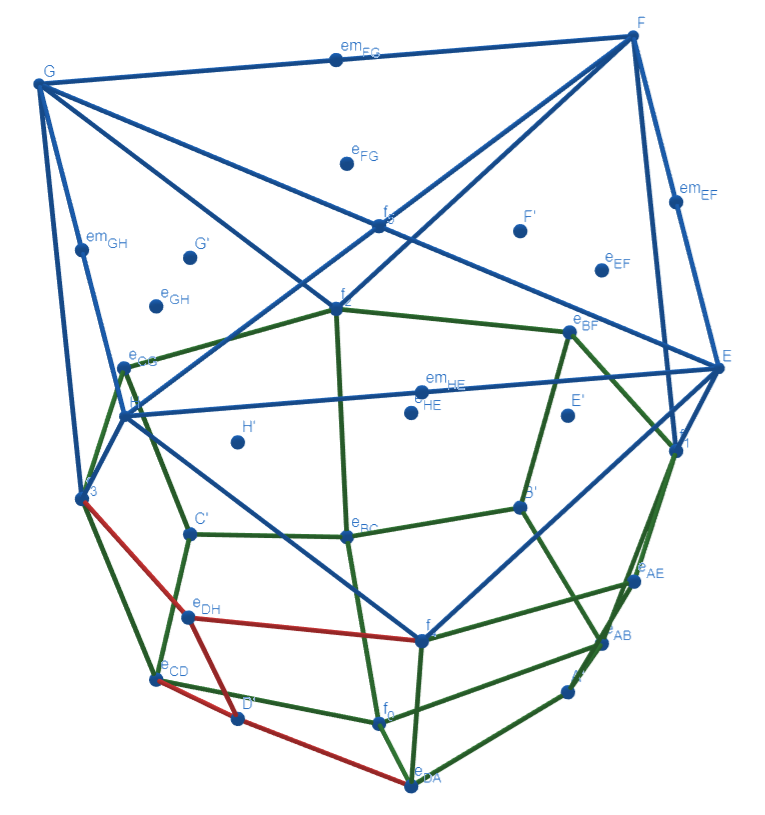
\includegraphics[width=0.8\textwidth]{images/cl-07-4.png}
\label{fig:cube7-4}
\end{figure}
\subsubsection{E \rightarrow E'}
\begin{figure}[H]
\caption{E' (GeoGebra link: \href{https://ggbm.at/kwqrtdzs}{https://ggbm.at/kwqrtdzs})}
\centering
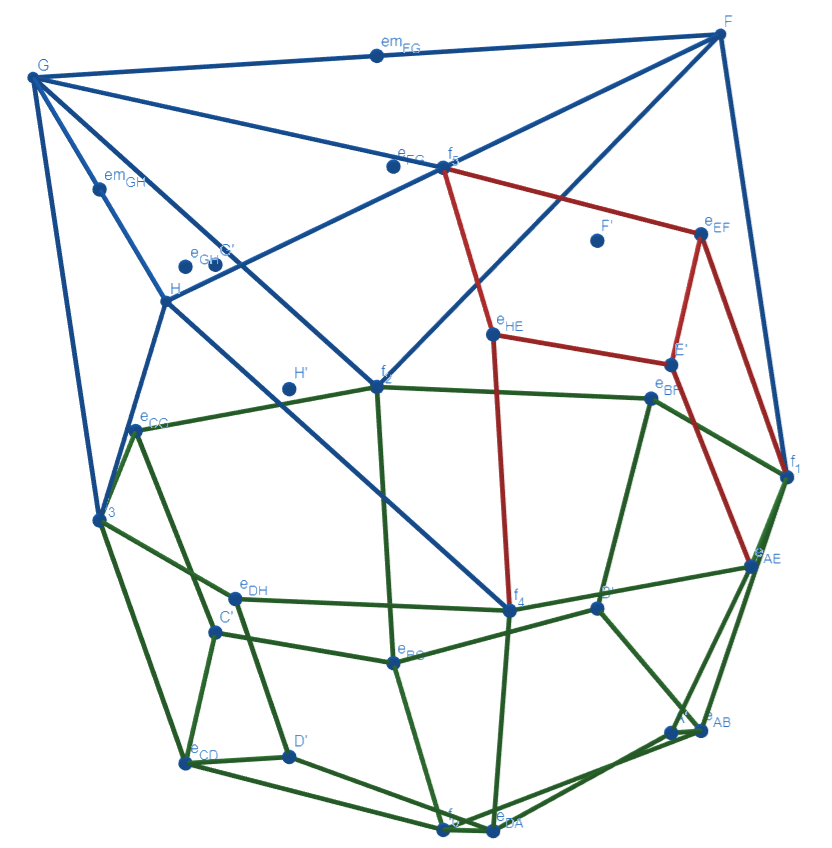
\includegraphics[width=0.8\textwidth]{images/cl-07-5.png}
\label{fig:cube7-5}
\end{figure}
\subsubsection{F \rightarrow F'}
\begin{figure}[H]
\caption{F' (GeoGebra link: \href{https://ggbm.at/gqnfxyjk}{https://ggbm.at/gqnfxyjk})}
\centering
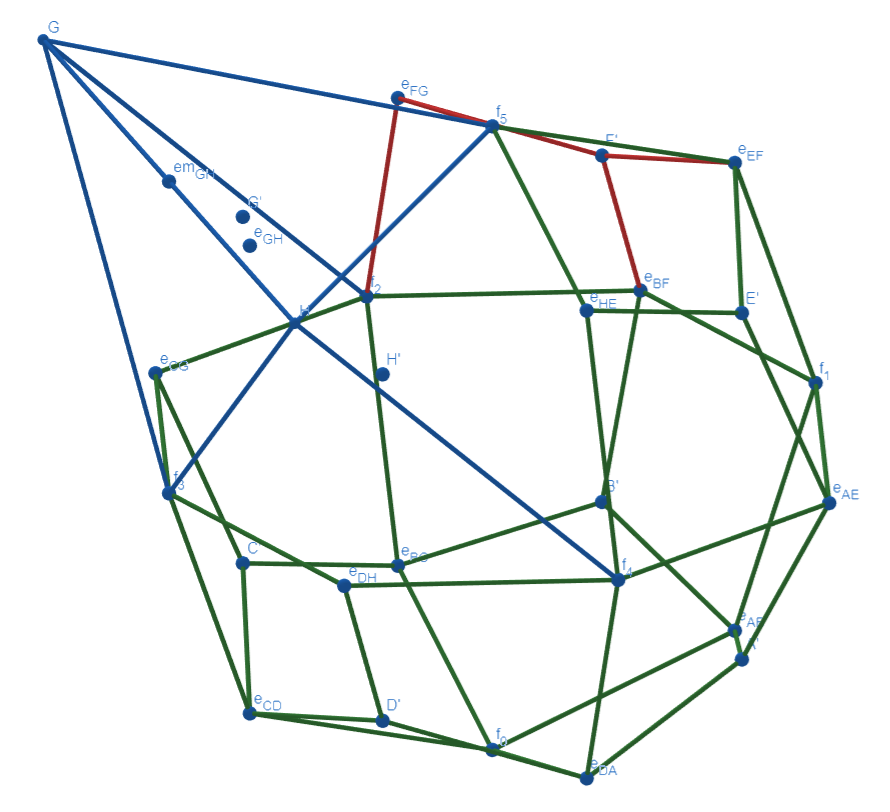
\includegraphics[width=0.8\textwidth]{images/cl-07-6.png}
\label{fig:cube7-6}
\end{figure}
\subsubsection{G \rightarrow G'}
\begin{figure}[H]
\caption{G' (GeoGebra link: \href{https://ggbm.at/exzncjsu}{https://ggbm.at/exzncjsu})}
\centering
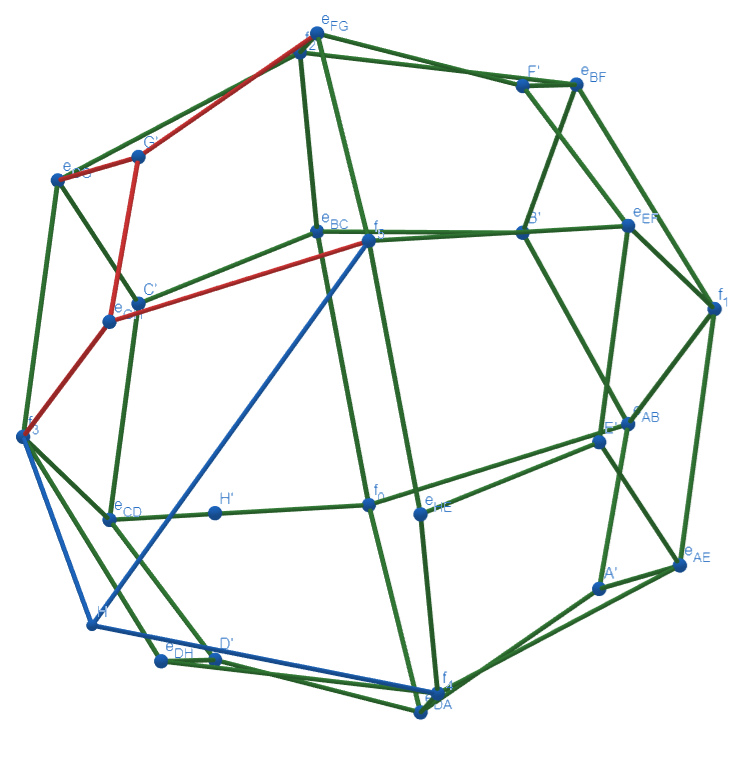
\includegraphics[width=0.8\textwidth]{images/cl-07-7.png}
\label{fig:cube7-7}
\end{figure}
\subsubsection{H \rightarrow H'}
\begin{figure}[H]
\caption{H' (GeoGebra link: \href{https://ggbm.at/nr3s6n4y}{https://ggbm.at/nr3s6n4y})}
\centering
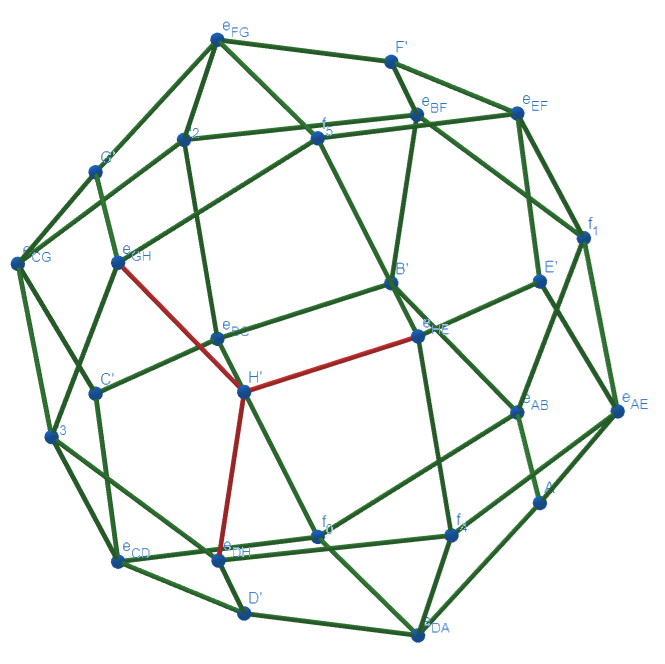
\includegraphics[width=0.8\textwidth]{images/cl-07-8.png}
\label{fig:cube7-8}
\end{figure}
\subsection{Finished sub division}
\begin{figure}[H]
\caption{Finished Catmull-Clark sub division (GeoGebra link: \href{https://ggbm.at/a4dng2bt}{https://ggbm.at/a4dng2bt})}
\centering
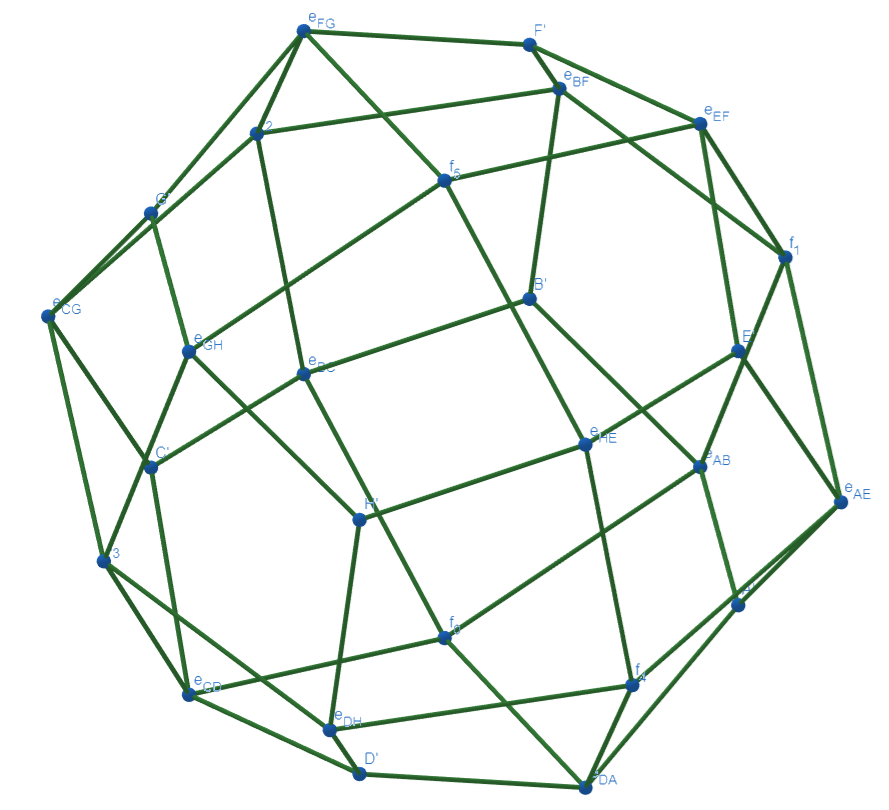
\includegraphics[width=0.8\textwidth]{images/cl-08.png}
\label{fig:cube8}
\end{figure}
\begin{figure}[H]
\caption{Finished Catmull-Clark sub division}
\centering
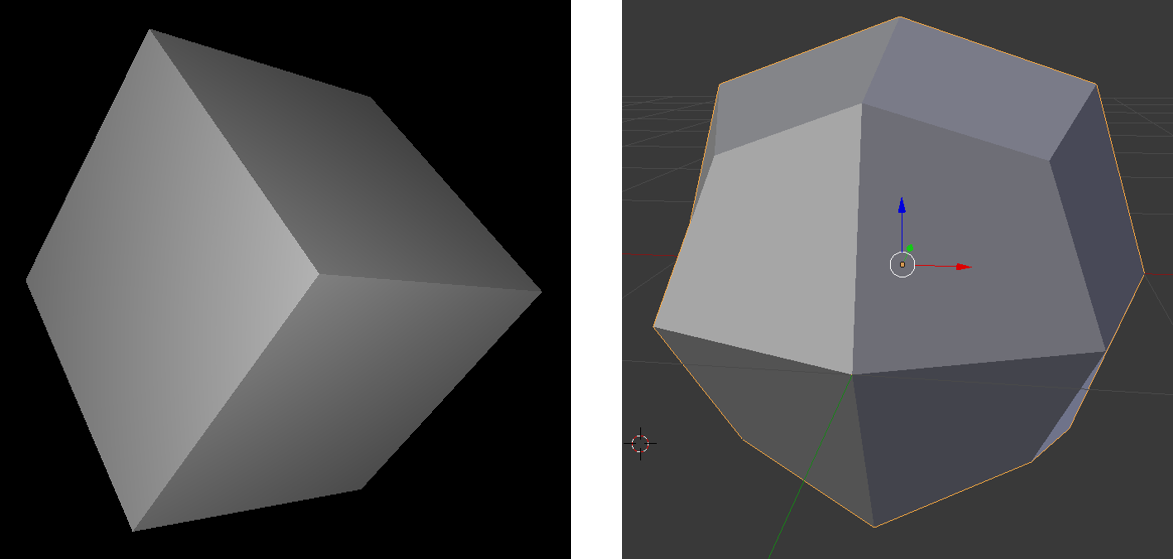
\includegraphics[width=1\textwidth]{images/cc-result.png}
\label{fig:cc-result}
\end{figure}
\section{Verification}
This section compares the manually calculated points with the computed values from JavaScript algorithm found on GitHub (\href{https://github.com/Erkaman/gl-catmull-clark}{https://github.com/Erkaman/gl-catmull-clark}). Table \ref{table:1} shows the vertex results. The results are the same but other vertex order, this is caused by internal structure of the algorithm.
\begin{center}
\begin{table}[!h]
\renewcommand{\arraystretch}{1.5}
    \caption{Left: manual calculation, right: algorithm results}
    \label{table:1}
    \begin{minipage}{.5\linewidth}
      \centering
        \begin{tabular}{ | r | c | c | c | }
    \hline
    vertex & x & y & z \\ \hline
    f_0 & 0 & 0 & 0 \\ \hline
    f_1 & 0 & -1 & 1 \\ \hline
    f_2 & 1 & 0 & 1 \\ \hline
    f_3 & 0 & 1 & 1 \\ \hline
    f_4 & -1 & 0 & 1 \\ \hline    
    f_5 & 0 & 0 & 2 \\ \hline
    e_{AB} & 0 & $ -\rfrac{3}{4} $ & $ \rfrac{1}{4} $ \\ \hline
    e_{BC} & $ \rfrac{3}{4} $ & 0 & $ \rfrac{1}{4} $ \\ \hline
    e_{CD} & 0 & $ \rfrac{3}{4} $ & $ \rfrac{1}{4} $ \\ \hline
    e_{DA} & $ -\rfrac{3}{4} $ & 0 & $ \rfrac{1}{4} $ \\ \hline
    e_{AE} & $ -\rfrac{3}{4} $ & $ -\rfrac{3}{4} $ & 1 \\ \hline    
    e_{BF} & $ \rfrac{3}{4} $ & $ -\rfrac{3}{4} $ & 1 \\ \hline
    e_{CG} & $ \rfrac{3}{4} $ & $ \rfrac{3}{4} $ & 1 \\ \hline    
    e_{DH} & $ -\rfrac{3}{4} $ & $ \rfrac{3}{4} $ & 1 \\ \hline
    e_{EF} & 0 & $ -\rfrac{3}{4} $ & $ \rfrac{7}{4} $ \\ \hline    
    e_{FG} & $ \rfrac{3}{4} $ & 0 & $ \rfrac{7}{4} $ \\ \hline
    e_{GH} & 0 & $ \rfrac{3}{4} $ & $ \rfrac{7}{4} $ \\ \hline    
    e_{HE} & $ -\rfrac{3}{4} $ & 0 & $ \rfrac{7}{4} $ \\ \hline
    A' & $ -\rfrac{5}{9} $ & $ -\rfrac{5}{9} $ & $ \rfrac{4}{9} $ \\ \hline
    B' & $ \rfrac{5}{9} $ & $ -\rfrac{5}{9} $ & $ \rfrac{4}{9} $ \\ \hline
    C' & $ \rfrac{5}{9} $ & $ \rfrac{5}{9} $ & $ \rfrac{4}{9} $ \\ \hline
    D' & $ -\rfrac{5}{9} $ & $ \rfrac{5}{9} $ & $ \rfrac{4}{9} $ \\ \hline
    E' & $ -\rfrac{5}{9} $ & $ -\rfrac{5}{9} $ & $ \rfrac{14}{9} $ \\ \hline    
    F' & $ \rfrac{5}{9} $ & $ -\rfrac{5}{9} $ & $ \rfrac{14}{9} $ \\ \hline
    G' & $ \rfrac{5}{9} $ & $ \rfrac{5}{9} $ & $ \rfrac{14}{9} $ \\ \hline    
    H' & $ -\rfrac{5}{9} $ & $ \rfrac{5}{9} $ & $ \rfrac{14}{9} $ \\ \hline
    \hline
  \end{tabular}
    \end{minipage}%
    \begin{minipage}{.5\linewidth}
      \centering
        \begin{tabular}{ | r | c | c | c | }
    \hline
    vertex & x & y & z \\ \hline
    D' & $ -\rfrac{5}{9} $ & $ \rfrac{5}{9} $ & $ \rfrac{4}{9} $ \\ \hline
    e_{CD} & 0 & $ \rfrac{3}{4} $ & $ \rfrac{1}{4} $ \\ \hline
    f_0 & 0 & 0 & 0 \\ \hline
    e_{DA} & $ -\rfrac{3}{4} $ & 0 & $ \rfrac{1}{4} $ \\ \hline
    C' & $ \rfrac{5}{9} $ & $ \rfrac{5}{9} $ & $ \rfrac{4}{9} $ \\ \hline    
    e_{BC} & $ \rfrac{3}{4} $ & 0 & $ \rfrac{1}{4} $ \\ \hline
    B' & $ \rfrac{5}{9} $ & $ -\rfrac{5}{9} $ & $ \rfrac{4}{9} $ \\ \hline
    e_{AB} & 0 & $ -\rfrac{3}{4} $ & $ \rfrac{1}{4} $ \\ \hline
    A' & $ -\rfrac{5}{9} $ & $ -\rfrac{5}{9} $ & $ \rfrac{4}{9} $ \\ \hline
    e_{BF} & $ \rfrac{3}{4} $ & $ -\rfrac{3}{4} $ & 1 \\ \hline
    f_1 & 0 & -1 & 1 \\ \hline    
    F' & $ \rfrac{5}{9} $ & $ -\rfrac{5}{9} $ & $ \rfrac{14}{9} $ \\ \hline
    e_{EF} & 0 & $ -\rfrac{3}{4} $ & $ \rfrac{7}{4} $ \\ \hline    
    E' & $ -\rfrac{5}{9} $ & $ -\rfrac{5}{9} $ & $ \rfrac{14}{9} $ \\ \hline
    e_{AE} & $ -\rfrac{3}{4} $ & $ -\rfrac{3}{4} $ & 1 \\ \hline    
    e_{CG} & $ \rfrac{3}{4} $ & $ \rfrac{3}{4} $ & 1 \\ \hline
    f_2 & 1 & 0 & 1 \\ \hline
    G' & $ \rfrac{5}{9} $ & $ \rfrac{5}{9} $ & $ \rfrac{14}{9} $ \\ \hline
    e_{FG} & $ \rfrac{3}{4} $ & 0 & $ \rfrac{7}{4} $ \\ \hline
    e_{DH} & $ -\rfrac{3}{4} $ & $ \rfrac{3}{4} $ & 1 \\ \hline    
    f_3 & 0 & 1 & 1 \\ \hline    
    H' & $ -\rfrac{5}{9} $ & $ \rfrac{5}{9} $ & $ \rfrac{14}{9} $ \\ \hline
    e_{GH} & 0 & $ \rfrac{3}{4} $ & $ \rfrac{7}{4} $ \\ \hline
    f_4 & -1 & 0 & 1 \\ \hline    
    e_{HE} & $ -\rfrac{3}{4} $ & 0 & $ \rfrac{7}{4} $ \\ \hline
    f_5 & 0 & 0 & 2 \\ \hline
    \hline
  \end{tabular}
    \end{minipage} 
\end{table}
\end{center}
\renewcommand{\arraystretch}{1}
\bibliographystyle{plain}
\bibliography{main}

\end{document}
